\documentclass[a4paper, 12pt]{article}

\usepackage[T1]{fontenc}
\usepackage[polish]{babel} 
\usepackage[utf8]{inputenc} 
\usepackage{indentfirst}
\let\lll\undefined
\usepackage{amssymb}
\usepackage{setspace}
\usepackage{fancyhdr}
\usepackage{graphicx} 

\pagestyle{fancy} 
\newcommand{\mainmatter}{\clearpage \cfoot{\thepage\ of \pageref{LastPage}}
\pagenumbering{arabic}}




\begin{document}
	\begin{titlepage}
		
		\begin{center}

    	\vspace{5cm}
    		\Large\textit{\textbf{SPECYFIKACJA IMPLEMENTACYJNA 
    		\\''WireWorld'' DLA JĘZYKA PROGRAMOWANIA JAVA}}\\ 
		\vspace{5cm}
		\end{center} 


	\end{titlepage}
\newpage
\mainmatter
\setlength{\headheight}{15pt}
\doublespacing
\tableofcontents
\newpage

	\section{Diagram klas}
		\begin{figure}[h]
			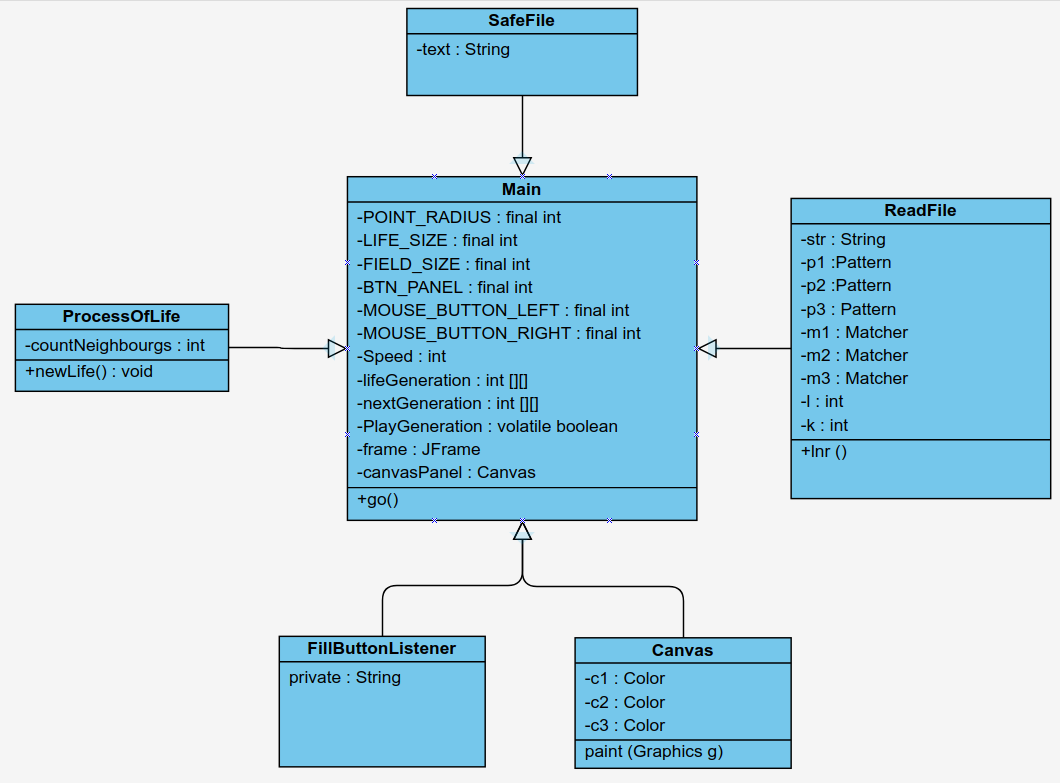
\includegraphics[width=\textwidth]{diagram.png}
			\caption{Diagram klas}
		\end{figure}		
\newpage
			\subsection{Opis diagramu} 
			\hspace*{1cm} Poniżej jest przedstawiony opis diagramu:\newline
			\hspace*{1cm} \texttt{Main} jest główną klasę. Klasa \texttt{Main} wiąże między sobą wszystkie poszczególne klasy w programie ''WireWorld''. \newline
			\hspace*{1cm} Metoda \texttt{void go()} zawiera cały interfejs graficzny oraz zarządzanie kliknięciem myszki i przesunięciem suwaka i odpowiada za \texttt{Start,Stop,NewGame}. Metoda \texttt{void go()} odpowiada za prędkość przesunięcia komórek. \newline
			\hspace*{1cm}W klasie \texttt{ReadFile} mamy \texttt{lnr} - LineNumberReader, który wczytuje poszczególne wartości z pliku \texttt{.txt}. \newline
			\hspace*{1cm}W klasie \texttt{Canvas} mamy metodę \texttt{public void paint(Graphics g)}, za pomocą której robimy graficzny interfejs dla pola i komórek.
\newpage
	\section{Opis metod/pakietów}
			\hspace*{1cm} Cały program został napisane w jednej klasie \texttt{Main.java}, bo na czas dzisiejszy innego rozwiązania problemu nie znaleźliśmy. \newline
			\hspace*{1cm} Kod programy jest napisany za pomocą dwóch tablic dwuwymiarowych i zmiennej typu \texttt{boolean} dla uruchomienia (Play) lub dla zatrzymania (Stop):
		\begin{itemize}
			\item \texttt{int[][] lifeGeneration},
			\item \texttt{int[][] nextGeneration},
			\item \texttt{volatile boolean PlayGeneration}.
		\end{itemize}
		\subsection{Klasa Main}
			\hspace*{1cm} Klasa \texttt{Main} zawiera w sobie klasy i następujące pola stałe:
		\begin{itemize}
			\item \texttt{final int POINT$\_$RADIUS} odpowiada za punkt radiusa,
			\item \texttt{final int LIFE$\_$SIZE} odpowiada za lewy rozmiar punktu,
			\item \texttt{final int FIELD$\_$SIZE} odpowiada za rozmiar okienka,
			\item \texttt{final int BTN$\_$PANEL} odpowiada za rozmiar paneli przycisków,
			\item \texttt{final int MOUSE$\_$BUTTON$\_$LEFT} odpowiada za lewy przycisk,
			\item \texttt{final int MOUSE$\_$BUTTON$\_$RIGHT} odpowiada za prawy przycisk,
			\item \texttt{int Speed} odpowiada za suwak prędkości, wartość maksymalnej prędkości.
		\end{itemize}
			
		\subsection{Metoda go()}
			\hspace*{1cm} Metoda \texttt{void go()} zawiera w sobie GUI i kod działania programu, które napisane poprzez bibliotekę \textbf{Swing}, jest stworzony \texttt{JFrame WireWorld} z odpowiednimi rozmiarami i wyglądem. Tak samo stworzony \texttt{JButton Play} dla uruchomienia działania programu.\newline
			\hspace*{1cm} Za pomocą \texttt{canvasPanel.addMouseListener} wyznaczamy naciski na myszkę, to znaczy, uzupełniamy wartościami:
		\begin{itemize}
			\item \texttt{MOUSE$\_$BUTTON$\_$LEFT},
			\item \texttt{MOUSE$\_$BUTTON$\_$RIGHT}.
		\end{itemize}		
			\hspace*{1cm} W tej metodzie  wyznaczamy suwak prędkości zależne od położenia wciśniętej myszki, za pomocą \texttt{public void stateChanged(ChangeEvent e)}.	
		
		\subsection{Metoda processOfLife}
			\hspace*{1cm} Metoda \texttt{void processOfLife()} liczy sąsiedztwa metodą Moore'a za pomocą dwóch dwuwymiarowych tablic. Tablica \texttt{lifeGeneration} odpowiada za stan teraźniejszy pozycji punktu, a tablica \texttt{nextGeneration} odpowiada za następującą generację punktów.
		
		\subsection{Metoda newLife}
			\hspace*{0,9cm} Metoda \texttt{void newLife()} oczyszcza całe plansze od wszystkich punktów i robi \texttt{newGame}.
		
		\subsection{Metoda saveFile}
			\hspace*{1cm} Metoda \texttt{void saveFile()} zapisuję wszystkie wygenerowane punkty do pliku w postaci: 
		\begin{verbatim}
			Field: 18, 20;
			ElectronTail: 19, 20;
			Field: 20, 20;
			ElectronHead: 21, 19;
			Field: 21, 20;
 		\end{verbatim}
 			\vspace{-0,8cm}
 			\hspace*{1cm} Gdzie \texttt{Field} to koordynata punktu, \texttt{ElectronTail} to ogon elektronu, \texttt{ElectronHead} to głowa elektronu. Z kolej wynika, że pole \texttt{Field} zawiera w~sobie \texttt{Diodę}.
		\subsection{Metoda readFile}
			\hspace*{1cm} Metoda \texttt{void readFile()} czyta punktu z pliku w postaci: 
		\begin{verbatim}
			Field: 18, 20;
			ElectronTail: 19, 20;
			Field: 20, 20;
			ElectronHead: 21, 19;
			Field: 21, 20;
 		\end{verbatim}
 			\vspace{-0,8cm}
 			\hspace*{1cm} Gdzie \texttt{Field} to koordynata punktu, \texttt{ElectronTail} to ogon elektronu, \texttt{ElectronHead} to głowa elektronu. Z kolej wynika, że pole \texttt{Field} zawiera w~sobie \texttt{Diodę}.
			
		\subsection{Pakiet}
			\hspace*{1cm} Cały program ''WireWorld'' jest napisany w \texttt{package gra}, bo zdecydowaliśmy, że w ten sposób będzie łatwej.
\newpage
	\section{Metodyka ''WireWorld''}
		\subsection{Zasady}
			\hspace*{1cm} Program ''WireWorld'' wykorzystuje zestaw zasad:
		\begin{itemize}
			\item Komórka pozostaje Pusta, jeśli była Pusta,
			\item Komórka staje się Ogonem elektronu, jeśli była Głową elektronu,
			\item Komórka staje się Przewodnikiem, jeśli była Ogonem elektronu
			\item Komórka staje się Głową elektronu tylko wtedy, gdy dokładnie 1 lub 2 sąsiadujące komórki są Głowami Elektronu,
			\item Komórka staje się Przewodnikiem w każdym innym wypadku.
		\end{itemize}			
		\subsection{Metoda sąsiedztw}			 
			 \hspace*{0,5cm}Program napisany za pomocą metody sąsiedztw Moore'a. W sąsiedztwie Moore'a mamy 8 przylegających komórek (znajdujących się: na południu, na południowym-zachodzie, na zachodzie, na północnym-zachodzie, na północy, na północnym-wschodzie, na wschodzie i na południowym-wschodzie). 
\newpage	
	\section{Opis GUI}
			\hspace*{1cm} Jest trochę opisany w metodzie \textbf{void go()}, ale tutaj bardziej szczegółowo:
		\begin{itemize}
			\item \texttt{JFrame} tworzy okienko o rozmiarze \texttt{500x570},
			\item \texttt{JFrame.EXIT$\_$ON$\_$CLOSE} odpowiada za wyłączenia programu przy nacisknięciu na czerwony suwak krzyż,
			\item \texttt{Canvas} tworzy panel do wykorzystywanie i wciśnięcia myszką, żeby pojawiały się diodę, punktu,
			\item \texttt{JSlider} tworzy liniowe regulatory (suwaki), które dają możliwość wyboru konkretnej wartości prędkości z zakresu od 1 do 700,
			\item \texttt{JButton Step} pokazuję generacje krok po kroku,
			\item \texttt{JButton Play} symuluje generacje z prędkością 350,
			\item \texttt{JButton Stop} zatrzyma działania kolejnych generacji,
			\item \texttt{JButton NewGame} wyczyszcza całe pole i zaczyna program od nowa,
			\item \texttt{JButton Save} zapisuje generacje do pliku z rozszerzeniem \texttt{.txt},
			\item \texttt{JButton Upload} otworzy plik \texttt{.txt} z odpowiednimi generacjami.
		\end{itemize}
		
		

\newpage	
	\section{Testowanie}
		\subsection{Użyte narzędzia}
			\subsubsection{AssertJ}
				\hspace*{1cm} Testy jednostkowe będą robione z wykorzystaniem biblioteki \textbf{AssertJ}, która pozwala na nagrywanie zatwierdzenia w Java-testów.

			\subsubsection{Maven}
				\hspace*{1cm} \textbf{Maven} — narzędzie automatyzujące budowę oprogramowania na platformę Java. Plik określający sposób budowy aplikacji nosi nazwę POM-u (ang. Project Object Model). W naszym programie będziemy wykorzystywać \textbf{Mavena} aby zapewnić przenośność kodu na poziomie deweloperskim. Poprzez użycie \textbf{Mavena} powstanie plik wynikowy z rozszerzeniem \texttt{.jar}.
\label{LastPage}~
\label{LastPageOfBackMatter}~		
\end{document}